%%%%%%%%%%%%%%%%%%%%%%%%%%%%%%%%%%%%%%%%%%%%%%%%%%%%%%%%%%%%%%%%%%%%%
% File Name:        imta_documentation
%
% Description:      documentation of the IMT Atlantique LaTeX Template.
%
% Note:             /
%
% Limitations:      /
%
% Errors:           None known
%
% Dependencies:     babel
%				    imta_core
%                   imta_extra
%                   isodate
%
% Author:          A. Foucault - armand.foucault@telecom-bretagne.eu
% Contributors:    B. Porteboeuf - benoit.porteboeuf@telecom-bretagne.eu
%
% University :     IMT Atlantique, Brest (France)
%
% TeX Environment: TeXLive + pdfLaTeX
%%%%%%%%%%%%%%%%%%%%%%%%%%%%%%%%%%%%%%%%%%%%%%%%%%%%%%%%%%%%%%%%%%%%
% !TeX TXS-program:compile = txs:///pdflatex/[--shell-escape]

\documentclass{report}
\usepackage{pdfpages}
    \usepackage{rotating}
\usepackage[italian]{babel}
\usepackage[italian]{isodate}

\usepackage{imta_core}
\usepackage{imta_extra}

\cleanlookdateon

\author{892539 $\cdot$ Dinato Simone}
\imtaAuthorShort{A. Ramolivaz \& S.Dinato \& A.Tomasin}
\date{891923 $\cdot$ Ramolivaz André \\892614 $\cdot$ Tomasin Alberto}
\title{EUResearchHub: Progresso in sinergia}
\subtitle{Report per il progetto di CT0006 - Basi di Dati}


\imtaSetIMTStyle

%%%%%%%%%%%%%%%%%%%%%%%%%%%%%%% 
%%%%%%%%%% BEGINNING %%%%%%%%%% 
\begin{document}

	
\imtaMaketitlepage

\tableofcontents

\newpage




%%%%%%%%%%%%%%%%%%%%%%%
%%%   IMTA   CORE   %%%
%%%%%%%%%%%%%%%%%%%%%%%
\chapter{Introduzione}

\phantom{This text will be invisible}\\
Questo documento descrive come abbiamo progettato e implementato EUResearchHub: una web application user-friendly per rendere possibile la valutazione interna dei progetti di ricerca proposti per il finanziamento da parte dell'Unione Europea per il progetto accademico del corso:\textit{ Basi di Dati $\cdo$ [CT0006] - Ca' Foscari Università di Venezia}.
\begin{imtaQuote}
Se vogliamo avere idee originali, dobbiamo investire nella ricerca. Non si tratta solo di investire nel settore privato, ma anche nel settore pubblico  $\cdot$ Elon Musk \end{imtaQuote}


\section{Contesto dell'applicazione}

EUResearchHub è un sistema che mira a rendere efficiente la gestione e la valutazione dei progetti di ricerca, offrendo una piattaforma accattivante e funzionale sia per i ricercatori che per i valutatori. Abbiamo scelto questo tema principalmente per la sua rilevanza e attualità nel panorama della ricerca e dell'istruzione superiore.\\
Nel corso degli anni, il contesto della ricerca scientifica è cambiato notevolmente. Con l'avvento dell'era digitale, la ricerca è diventata sempre più interconnessa e collaborativa, permettendo ai ricercatori di tutto il mondo di lavorare insieme per risolvere problemi complessi. Tuttavia, questo cambiamento ha anche portato ad un aumento della competizione per i finanziamenti di ricerca, soprattutto da parte dell'Unione Europea, che è uno dei principali finanziatori di progetti di ricerca a livello globale.\\
Negli ultimi anni, l'Unione Europea ha lanciato diversi programmi di finanziamento, come Orizzonte 2020 e il suo successore, Orizzonte Europa, che hanno l'obiettivo di sostenere la ricerca e l'innovazione in diversi settori, come la salute, l'energia, l'ambiente e l'istruzione. Per accedere a questi fondi, le istituzioni di ricerca devono sottoporre i propri progetti a processi di valutazione rigorosi e competitivi.\\
In questo contesto, è fondamentale che le istituzioni di ricerca dispongano di strumenti efficaci per gestire e valutare i progetti di ricerca internamente, al fine di aumentare le possibilità di ottenere finanziamenti. EUResearchHub è stata concepita proprio per rispondere a questa necessità, fornendo una piattaforma che facilita la comunicazione e la collaborazione tra ricercatori e valutatori, permettendo loro di lavorare insieme in modo efficiente per migliorare la qualità dei progetti di ricerca proposti.\\


\section{Funzionalità principali}
\phantom{This text will be invisible}\\
Nel progettare EUResearchHub, abbiamo posto particolare enfasi sull'offerta di funzionalità che consentano una gestione efficiente e trasparente dei progetti di ricerca, facilitando il processo di valutazione e promuovendo una comunicazione efficace tra ricercatori e valutatori tramite un sistema di messaggistica e storico dei documenti. \\
A tal proposito è importante definire fin da subito definire due grandi aree. Una è quella riguardante il ricercatore e tutte le sue funzionalità mentre l’altra riguarda è legata al valutatore. \\
In questa sezione, ci concentreremo sulle tre funzionalità chiave per ogni area: la gestione dei progetti di ricerca, il processo di valutazione, lo storico delle modifiche e l'interazione tra ricercatori e valutatori.

%% Sectioning
\subsection{Gestione dei progetti di ricerca}
La gestione dei progetti di ricerca è una componente fondamentale per EuResearchHub. Il sistema è stato progettato per consentire ai ricercatori di creare e visualizzare facilmente nuovi progetti, inserendo informazioni pertinenti, come il titolo e la descrizione del progetto o aggiungere anche partecipanti al progetto.  Una volta creato il progetto, i ricercatori possono anche caricare documenti in formato PDF, come il piano di gestione dei dati, i materiali etici che verranno sottoposti ai valutatori durante processo di valutazione. I valutatori quindi non potranno aggiungere utenti al progetto, creare nuovi progetti e caricare documenti per gli stessi.\\
\subsection{Processo di valutazione e storico modifiche}
Una volta che i progetti di ricerca sono stati creati e sottomessi per la valutazione, i valutatori possono accedervi per valutarli. Il processo di valutazione è stato progettato per essere il più trasparente e approfondito ma allo stesso minimal possibile. I valutatori possono scaricare i documenti relativi al progetto, leggerli, analizzarli, e commentarli quindi creare un report di valutazione per ogni documento e caricarlo nuovamente sulla piattaforma per renderlo visibile ai ricercatori interessati. Questo report può includere commenti generali sul progetto, suggerimenti per miglioramenti e valutazioni specifiche per ogni documento allegato.\\
Una caratteristica importante del sistema è la possibilità di tracciare lo storico delle modifiche dei documenti e quindi dei progetti sottomessi. Ogni volta che un ricercatore apporta modifiche ad un documento e lo carica nel sistema EUResearchHub registra una nuova versione, mantenendo una copia della versione precedente. Questo permette sia ai ricercatori che ai valutatori di monitorare l'evoluzione del progetto nel tempo e di comprendere come le modifiche apportate abbiano influito sulla valutazione finale del progetto.\\
Lo storico delle modifiche è particolarmente utile nei casi in cui i valutatori richiedono modifiche ai progetti prima di approvarli. In questi casi, i ricercatori possono utilizzare lo storico delle versioni per confrontare le diverse versioni del progetto e identificare le aree in cui è necessario apportare miglioramenti. Per quanto concerne il processo di valutazione,  lo status come indicato potrà assumere il valori ma questi valori possono cambiare se tutti i documenti inseriti dal ricercatore sono stati valutati.  Entrambi gli utenti possono visionare la percentuale dei documenti valutati in corso e quanti ne mancano indicativamente tramite l'evaluation progress bar. 

\subsection{Interazione tra ricercatori e valutatori}
Insieme allo storico dei documenti la comunicazione tra ricercatori e valutatori è un aspetto cruciale per garantire un processo di valutazione efficace e monitorare il ciclo di vita di un progetto. EUResearchHub è dotata di una componente di messaggistica per ogni progetto che consente ai ricercatori e ai valutatori di interagire direttamente all'interno della piattaforma. Questa funzionalità consente ai ricercatori di richiedere chiarimenti sui report di valutazione, suggerimenti su come migliorare i loro progetti e informazioni aggiuntive sui requisiti specifici dei finanziamenti. Allo stesso tempo, i valutatori possono rispondere alle domande dei ricercatori in modo anonimo, garantendo l'obiettività e l'imparzialità del processo di valutazione.\\
I valutatori possono utilizzare questa funzione per fornire feedback specifico e mirato sui documenti, ad esempio evidenziando passaggi che richiedono chiarimenti o suggerendo modifiche al testo. Questi messaggi possono essere utilizzati dai ricercatori per apportare miglioramenti ai loro progetti e dai valutatori per fare riferimento a punti specifici nei loro report di valutazione (ad esempio, "si veda la nota a pagina 4").\\


\section{Obiettivi e scopo del documento}

In questo documento, si spiega come abbiamo progettato e modellato la base di dati partendo dalla raccolta ed analisi dei requisiti fino alla progettazione fisica con particolare enfasi sul controllo degli accessi e integrità dei dati per poi passare a descrivere l'implementazione del back-end e del front-end ed infine concludere con una panoramica generale del processo di sviluppo e il contributo individuale dei membri del gruppo di lavoro.\\


\chapter{Progettazione della base di dati}
\phantom{This text will be invisible}\\
L'efficacia di EUResearchHub per la valutazione interna dei progetti di ricerca dipende in gran parte dalla qualità e dall'efficienza della base di dati che ne supporta il funzionamento. In questo capitolo, ci concentreremo sulla progettazione e modellazione della base di dati, analizzando le varie fasi del processo, tra cui la raccolta e l'analisi dei requisiti, la progettazione concettuale, logica e fisica, e le considerazioni relative all'integrità dei dati, al controllo degli accessi e alle performance del sistema.

\section{Raccolta ed analisi dei requisiti}
La fase di raccolta ed analisi dei requisiti è stato uno dei più importanti pilastri per comprendere e definire le specifiche del sistema. In questa fase embrionale, abbiamo identificato le esigenze degli utenti e le funzionalità che la base di dati deve supportare per garantire il corretto funzionamento di tutto il sistema. 
\subsection{Quadro generale}
Come già accennato precedentemente EURsearchHub ha il compito di fornire una piattaforma di interazione tra ricercatori e valutatori per la valutazione interna dei progetti di ricerca. Il sistema deve quindi essere in grado di gestire progetti, documenti, messaggi e report di valutazione, oltre a fornire supporto per l'autenticazione e l'autorizzazione degli utenti.\\
Quindi, analizzando attentamente il problema le entità chiave individuate sono:

\begin{itemize}
    \item \imtaInlinecode{latex}{project}: contiene informazioni sui progetti di ricerca, come il titolo, lo stato (approvato, sottomesso per valutazione, richiede modifiche, non approvato), la descrizione e la data di creazione.
    \item \imtaInlinecode{latex}{evaluation_windows}: rappresenta le finestre temporali in cui i progetti possono essere valutati, con date di inizio e fine.
        \item \imtaInlinecode{latex}{messages}: contiene i messaggi scambiati tra ricercatori e valutatori riguardo ai progetti.
        
    \item \imtaInlinecode{latex}{documents} e  \imtaInlinecode{latex}{document_versions}: gestiscono i documenti associati ai progetti e le loro diverse versioni.

    \item \imtaInlinecode{latex}{document_types}: classifica i diversi tipi di documenti utilizzati nel sistema. Si ipotizza che vi siano dei tipi di documento pre-stabiliti dall'ente che saranno poi i soli tipi di documenti che un ricercatore potrà andare a caricare. 

    \item \imtaInlinecode{latex}{users}: evaluators e researchers che contengono informazioni sugli utenti del sistema, come nome, cognome, password ed e-mail.
    
    
    \item \imtaInlinecode{latex}{evaluation_reports}: archivia i report di valutazione generati dai valutatori per i documenti dei progetti di ricerca.


    \end{itemize}


\subsection{Vincoli preliminari}
Definite le entità chiave risulta fondamentale inserire dei vincoli per garantire l'integrità e coerenza dei dati che andremo ad inserire. Nel nostro contesto, assicurarsi che i dati siano accurati e coerenti è fondamentale per evitare errori nella valutazione e facilitare il processo decisionale.  Più in dettaglio i vincoli necessari individuati in questa prima fase sono stati:\\
\begin{itemize}
\item Vincolo sulla tabella \imtaInlinecode{latex}{evaluation_windows}: necessario per assicurarsi che la data di inizio sia sempre inferiore o uguale alla data di fine. Questo vincolo permette di prevenire la creazione di finestre di valutazione con date illogiche o errate, garantendo che le date siano coerenti e rispettino un ordine temporale corretto.

\item Vincoli sulla lunghezza delle password per le due tipologie di users \imtaInlinecode{latex}{researchers} ed \imtaInlinecode{latex}{evaluators}: necessari a garantire che le password degli utenti abbiano una lunghezza minima di 8 caratteri. Questo requisito aumenta la sicurezza degli account, riducendo la probabilità di accessi non autorizzati attraverso attacchi brute-force o altre tecniche di hacking. Sebbene questo controllo possa essere fatto anche dal back-end implementarlo anche nella base di dati permette di centralizzare il vincolo.

\item Vincoli sull'email per \imtaInlinecode{latex}{researchers} ed \imtaInlinecode{latex}{evaluators}: necessari per assicurarsi che gli indirizzi email siano unici, validi e rispettino il formato standard delle email. Questo vincolo previene l'inserimento di indirizzi email non validi o errati, garantendo una corretta comunicazione tra i ricercatori e i valutatori. 
    \end{itemize}
\subsection{Ruoli}
Un altro step necessario per proseguire con la raccolta ed analisi dei requisiti è individuare i ruoli e le politiche di autorizzazione. Questo è fondamentale per garantire la sicurezza e la corretta separazione delle responsabilità all'interno di una web app. Nel caso di EUResearchHub, abbiamo definito tre ruoli principali: \imtaInlinecode{latex}{Admin}, \imtaInlinecode{latex}{Researcher} e \imtaInlinecode{latex}{Evaluator}. Ognuno di questi ruoli dovrà avere privilegi e restrizioni specifici per garantire che gli utenti possano accedere e modificare solo le informazioni pertinenti alle loro funzioni.\\
Implementare ruoli ben definiti e separati ci permette di ottenere una maggiore sicurezza, una riduzione del rischio di abusi o accessi non autorizzati e una migliore organizzazione delle responsabilità all'interno del nostro sistema. \\
Da una prima analisi del problema otteniamo il seguente diagramma di autorizzazioni:
\begin{center}
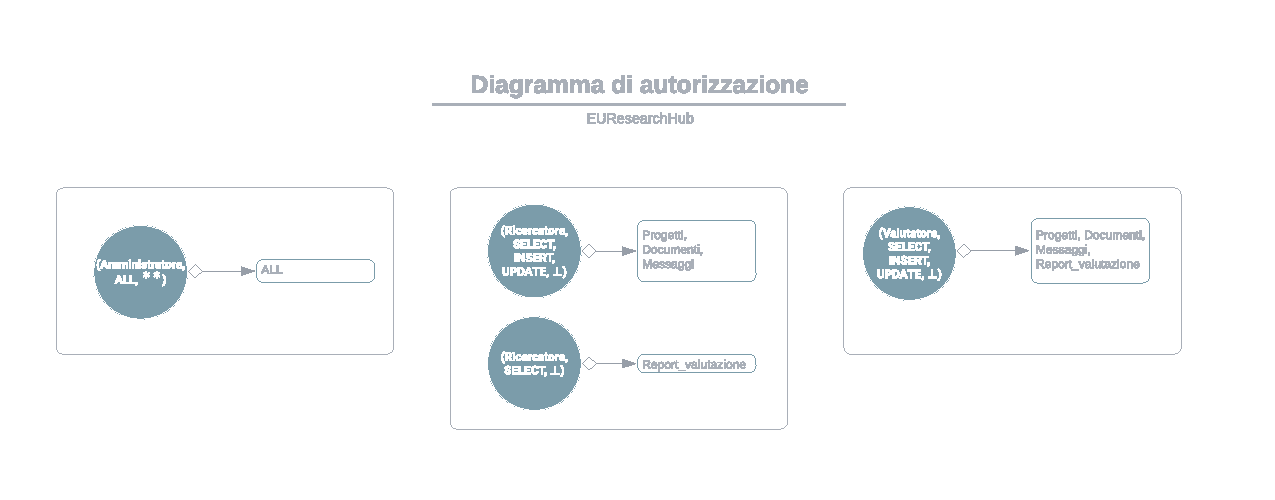
\includegraphics[scale = 0.7]{1.pdf}
\end{center}
Nel contesto descritto, non sembra necessario inserire ereditarietà o delega di permessi tra i ruoli, motivo per cui nel diagramma soprastante i nodi non sono legati tra di essi. Ogni ruolo ha responsabilità e permessi molto specifici e distinti, e non sembra esserci un caso d'uso in cui un ruolo avrebbe bisogno di ereditare i permessi di un altro ruolo.\\


\section{Progettazione concettuale}

Dopo l'analisi e raccolta dei requisiti il secondo pilastro necessario per la progettazione e modellazione del nostro database è la progettazione concettuale. Essa consente di strutturare gli elementi chiave del sistema prima identificati. Nel nostro caso, è stato utilizzato Lucidchart per sviluppare un modello ad oggetti che rappresenta le tabelle, le relazioni, i vincoli e le invarianti, fornendo una panoramica comprensiva e astratta dell'architettura del database.\\
Nel modello concettuale, le tabelle rappresentano le entità principali del sistema, come i ricercatori, i valuatori, i progetti, i documenti e così via. Le relazioni tra queste entità sono state modellate con parzialità e molteplicità, indicando come le diverse entità interagiscono tra loro e quali sono le dipendenze tra di esse.\\
Gli invarianti sono stati evidenziati infondo alle tabelle interessate per garantire l'integrità e la consistenza dei dati. Ad esempio, alcuni dei vincoli menzionati in precedenza, come il controllo sulla lunghezza delle password e il formato degli indirizzi email, sono stati inclusi nel modello per assicurare che i dati inseriti nel sistema rispettino le regole e standard.
\subsection{Schema ad oggetti}
\begin{sidewaysfigure}
\centering
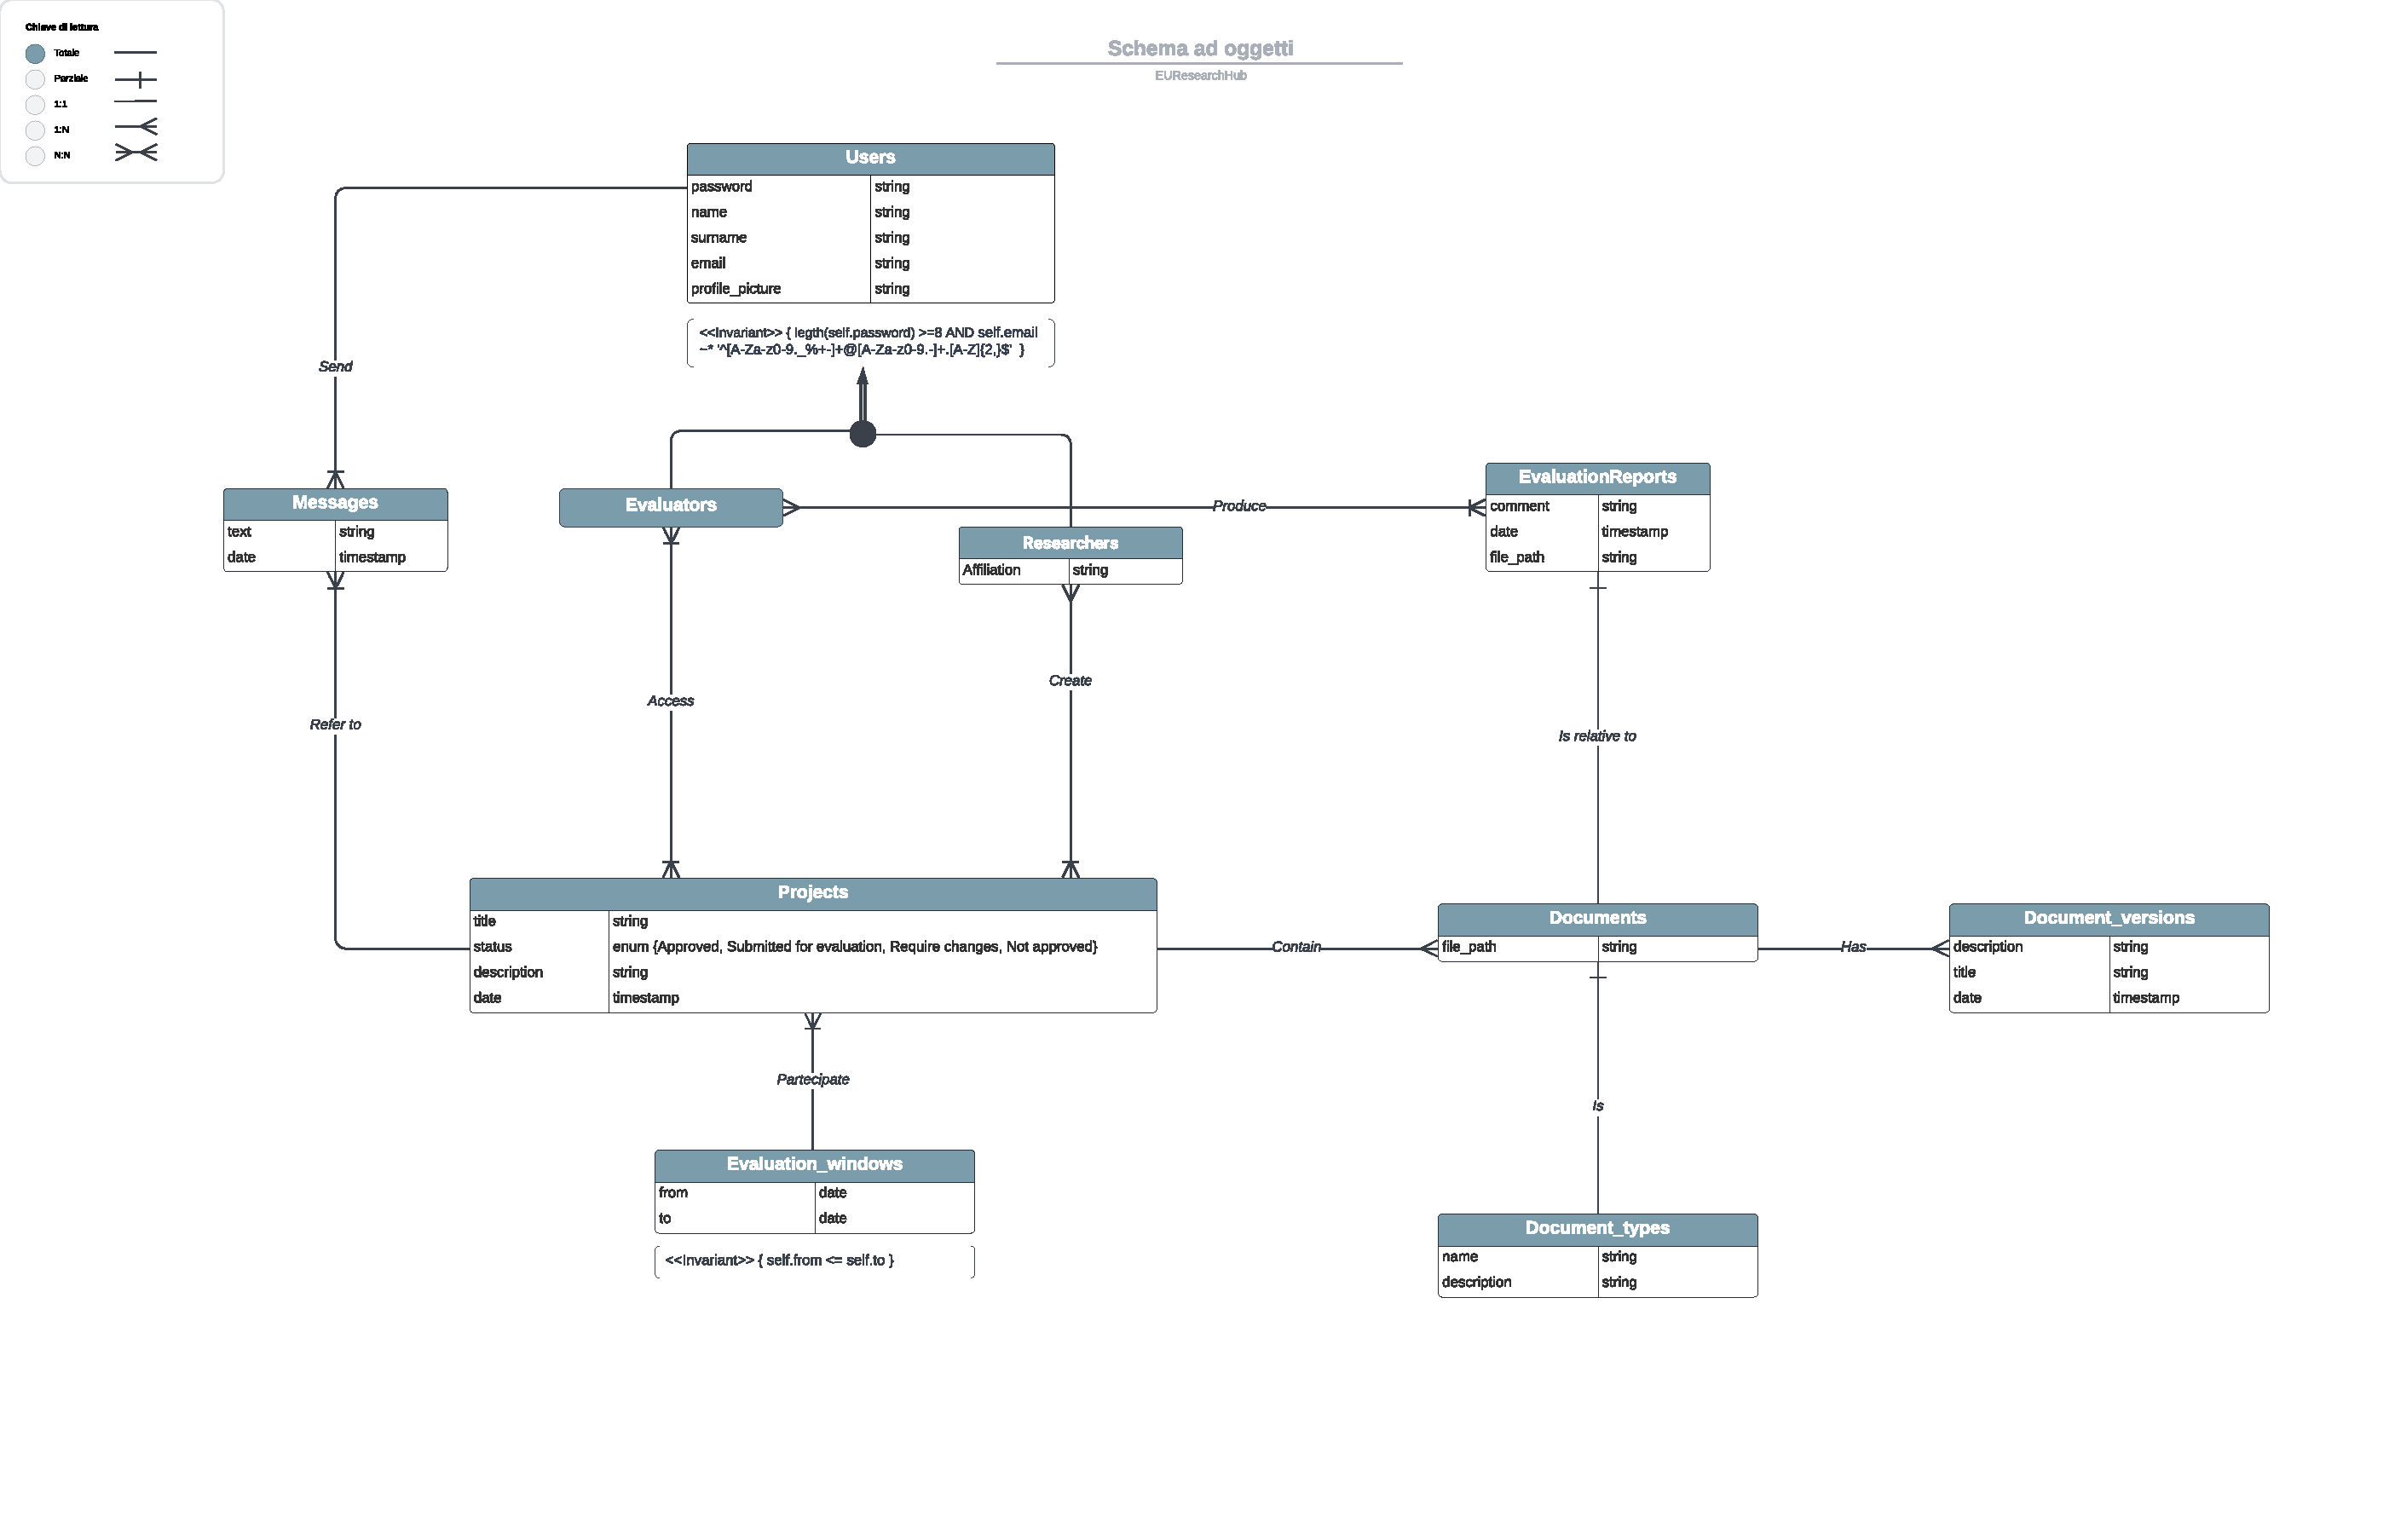
\includegraphics[width=1.00\textwidth]{Schema a oggetti.pdf}
\caption{Schema ad oggetti}
\end{sidewaysfigure}
\newpage
\subsection{Giustificazione delle decisioni progettuali}
Di seguito sono riportate le giustificazioni delle principali decisioni progettuali per garantire che il sistema fosse scalabile, efficiente e facile da mantenere:
\begin{itemize}
\item \textbf{Utilizzo di tipi enum:} Per rappresentare lo status dei progetti, creeremo un tipo enumerato \imtaInlinecode{latex}{enum_status}. Questo garantisce che solo i valori predefiniti possano essere inseriti nella colonna status della tabella \imtaInlinecode{latex}{projects}, garantendo la consistenza dei dati e facilitando le query sullo stato dei progetti.

\item \textbf{Definita una relazione di sottoclasse:} Sono state definite due sottoclassi partizione \imtaInlinecode{latex}{researchers} e \imtaInlinecode{latex}{evaluators} che ereditano gli attributi da \imtaInlinecode{latex}{users} per evitare eventuali ridondanze e permettere durante la progettazione logica di effettuare l'implementazione corretta.

\item \textbf{Suddivisione delle informazioni in tabelle separate:} Al fine di garantire la normalizzazione del database e ridurre la ridondanza dei dati, le informazioni sono state suddivise in tabelle separate. Ad esempio, le informazioni sui documenti e le loro versioni sono state divise nelle tabelle \imtaInlinecode{latex}{documents} e \imtaInlinecode{latex}{document_versions}, permettendo di gestire più versioni di uno stesso documento in modo efficiente. In maniera analoga anche le \imtaInlinecode{latex}{evaluation_windows} vengono salvate in una tabella separata da \imtaInlinecode{latex}{projects}.

\item \textbf{Utilizzo di invarianti:} già accennate in precedenza.

\end{itemize}


\section{Progettazione logica}
Ora analizziamo la fase intermedia della nostra modellazione: La progettazione logica. 
In questa fase, abbiamo tradotto il modello concettuale ad oggetti in uno schema logico che è stato utilizzato poi durante la creazione del database. La progettazione logica è essenziale per diverse ragioni:
\begin{enumerate}
\item Consente di identificare e risolvere eventuali problemi nella struttura dei dati prima di passare alla progettazione fisica.
\item Semplifica la mappatura tra il modello concettuale e il modello fisico, riducendo il rischio di errori e migliorando la coerenza dei dati.
\item Fornisce un'opportunità per ottimizzare le prestazioni del database, ad esempio selezionando gli indici appropriati e creando viste materializzate per migliorare l'efficienza delle query che si andranno ad implementare durante la progettazione fisica.
\end{enumerate}

\subsection{Schema logico}
\begin{sidewaysfigure}
\centering
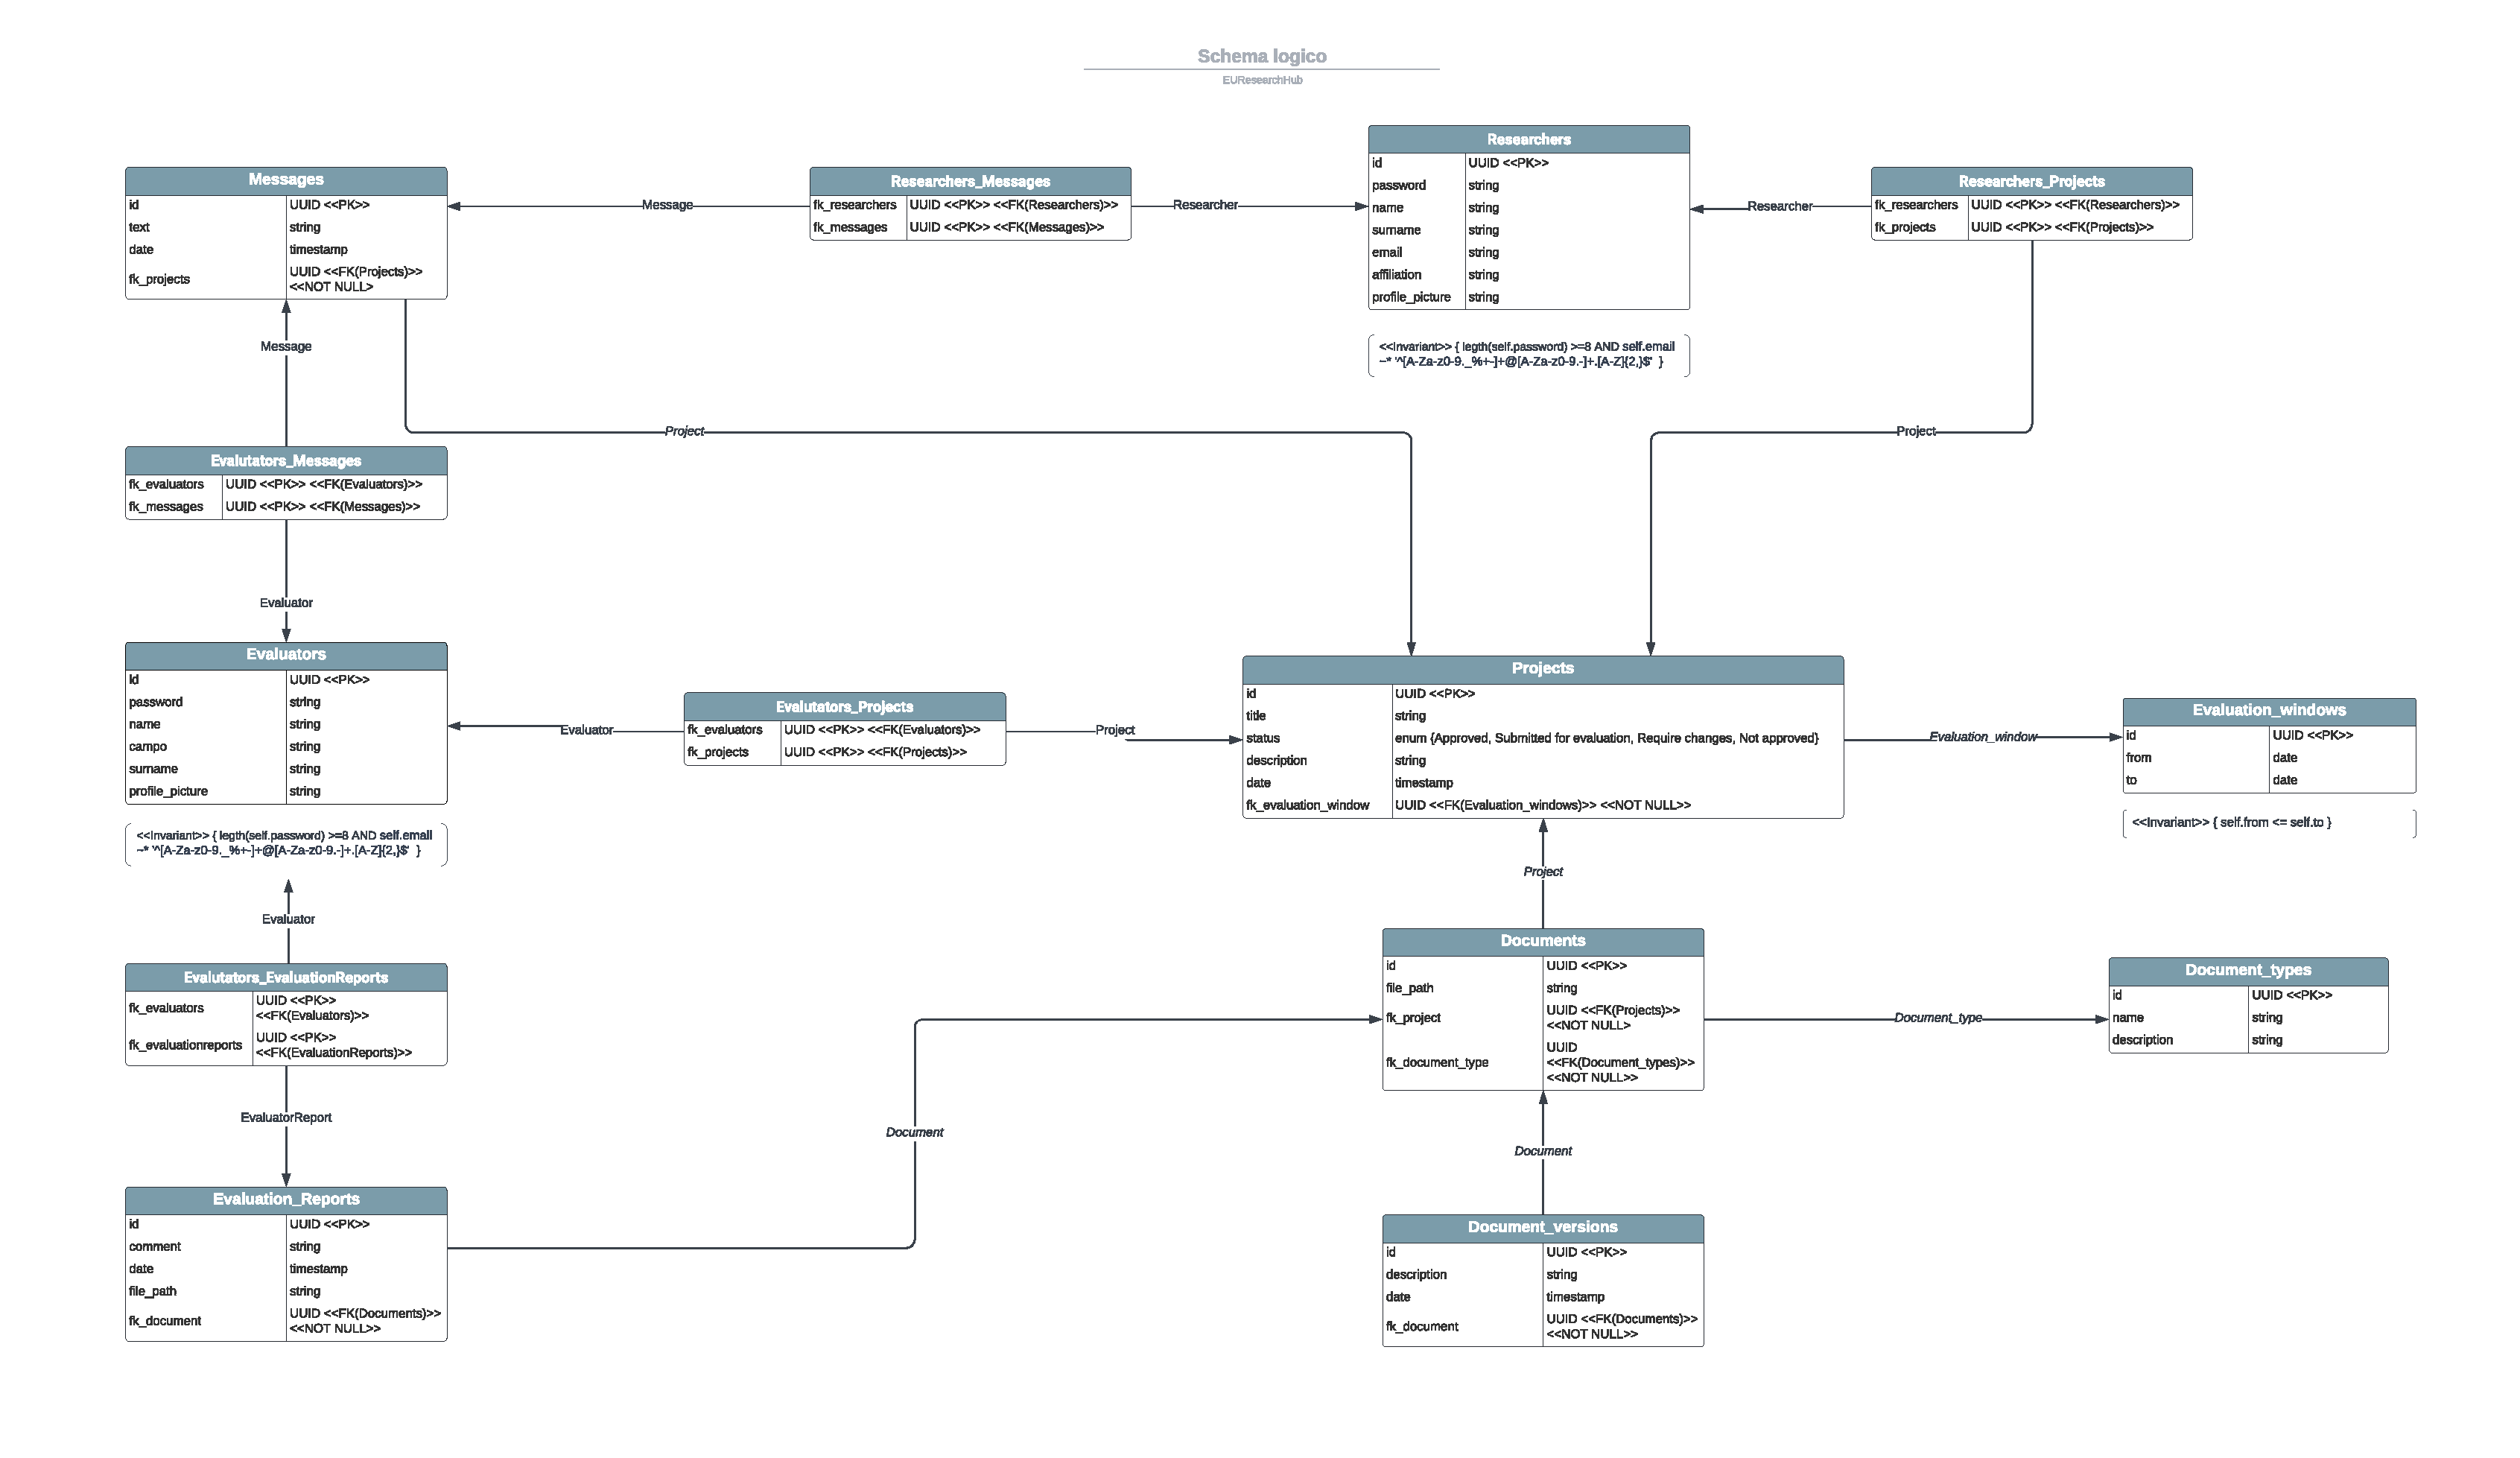
\includegraphics[width=1.00\textwidth]{Schema logico.pdf}
\caption{Schema logico}
\end{sidewaysfigure}
\newpage
\subsection{Giustificazione delle decisioni progettuali}
Di seguito sono riportate le giustificazioni di alcune delle decisioni chiave per questa fase:
\begin{itemize}

\item\textbf{ Tradotta la relazione di sottoclasse tramite partizionamento orizzontale:} Dalla gerarchia iniziale si è arrivati a suddividere le due sottoclassi partizione \imtaInlinecode{latex}{researchers} e \imtaInlinecode{latex}{evaluators}  in due tabelle a se stanti che ereditano gli attributi da \imtaInlinecode{latex}{users} poiché non si voleva complicare maggiormente la vista di tutti gli elementi della super classe tramite partizionamento verticale e neanche generalizzare troppo utilizzando una discriminante e ragruppando tutti gli attributi nella tabella unica \imtaInlinecode{latex}{users}.

\item \textbf{Chiavi esterne e relazioni:} Sono state utilizzate chiavi esterne per stabilire relazioni tra le diverse tabelle, garantendo l'integrità referenziale e semplificando le query tra tabelle correlate. Ad esempio, la tabella \imtaInlinecode{latex}{documents} ha una chiave esterna che fa riferimento alla tabella \imtaInlinecode{latex}{projects}, indicando a quale progetto appartiene ciascun documento.

\item \textbf{Utilizzo di tabelle intermedie per relazioni molti-a-molti:} Per gestire le relazioni molti-a-molti tra entità, sono state create tabelle intermedie, come \imtaInlinecode{latex}{researchers_projects} e \imtaInlinecode{latex}{evaluators_messages}. Queste tabelle consentono di associare più ricercatori a più progetti e più messaggi a più valutatori, garantendo la flessibilità del sistema e semplificando le query tra tabelle correlate.

\item \textbf{Inserito \imtaInlinecode{latex}{id} univoco per ogni tabella:} Ogni tabella è caratterizzata da un ID univoco sotto forma di intero auto incrementato.

\item \textbf{Inserito vincolo \imtaInlinecode{latex}{UNIQUE} sulle mail:} Ogni utente è caratterizzata da un email che deve essere univoco.


\end{itemize}


\section{Progettazione fisica}
LA progettazione fisica presenta l'ultima stazione per completare questa prima parte di attività.  Vista l'analisi a 360° del database, e di come dovrebbe funzionare l'applicativo non resta che applicare le osservazioni fatte su DBeaver. I costrutti per la creazione si basano sul linguaggio PostgreSQL.
\subsection{Istruzioni \texttt{SQL}}
Per le istruzioni SQL di creazione della base di dati si veda allegato \imtaInlinecode{latex}{dump.sql}. 

\subsection{Specifiche integrità dei dati}
Definite le tabelle in SQL chiave risulta fondamentale inserire i vincoli individuati durante la raccolta ed analisi dei requisiti e aggiungerne nuovi individuati durante la progettazione.  
Più in dettaglio i vincoli definitivi implementati in PosgreSQL sono stati:\\
\phantom{This text will be invisible}\\
Vincolo sulla tabella \imtaInlinecode{latex}{evaluation_windows}
\begin{imtaCode}{PostgreSQL}
ALTER TABLE "EUResearchHub".evaluation_windows
ADD CONSTRAINT evaluation_windows_dates_check CHECK ("from" <= "to");
\end{imtaCode}
\phantom{This text will be invisible}\\
Vincoli sulla lunghezza delle password per le due tipologie di users \imtaInlinecode{latex}{researchers} ed \imtaInlinecode{latex}{evaluators}
\begin{imtaCode}{PostgreSQL}
ALTER TABLE "EUResearchHub".researchers
ADD CONSTRAINT researchers_password_length_check CHECK (LENGTH("password") >= 8);

ALTER TABLE "EUResearchHub".evaluators
ADD CONSTRAINT evaluators_password_length_check CHECK (LENGTH("password") >= 8);
\end{imtaCode}
\phantom{This text will be invisible}\\
Vincoli sull'email per \imtaInlinecode{latex}{researchers} ed \imtaInlinecode{latex}{evaluators}:
\begin{imtaCode}{PostgreSQL}
ALTER TABLE "EUResearchHub".researchers
ADD CONSTRAINT researchers_email_check CHECK (email ~* '^[A-Za-z0-9._%+-]+@[A-Za-z0-9.-]+\.[A-Z]{2,}$');

ALTER TABLE "EUResearchHub".evaluators
ADD CONSTRAINT researchers_email_check CHECK (email ~* '^[A-Za-z0-9._%+-]+@[A-Za-z0-9.-]+\.[A-Z]{2,}$');
\end{imtaCode}
Il vincolo utilizza una regex (espressione regolare). Le espressioni regolari sono potenti strumenti utilizzati per cercare e confrontare stringhe di testo basate su modelli specifici.  Per comprenderne meglio il funzionamento possiamo dividere la stringa in 4 parti: 

\begin{enumerate}
\item \textbf{\^[A-Za-z0-9.\_\%+-]+}: questa parte dell'espressione indica che l'indirizzo email deve iniziare (\^) con una sequenza di almeno un carattere (+) che può essere una lettera maiuscola o minuscola, un numero, un punto, un underscore, un simbolo di percentuale, un simbolo più o un simbolo meno.
\item \textbf{@}: questo simbolo indica che, dopo la sequenza iniziale di caratteri, deve essere presente il simbolo "@" che separa la parte locale dell'indirizzo email dal dominio.
\item \textbf{[A-Za-z0-9.-]+}: questa parte dell'espressione indica che, dopo il simbolo "@", deve esserci una sequenza di almeno un carattere (+) che può essere una lettera maiuscola o minuscola, un numero, un punto o un trattino. Questa sequenza rappresenta il dominio dell'indirizzo email (ad esempio, "gmail.com" o "example.org").
\item \textbf{ \.[A-Z]{2,}\$}: questa parte finale dell'espressione indica che, dopo il dominio, deve essere presente un punto seguito da almeno due lettere maiuscole o minuscole ({2,}). Questa sequenza rappresenta il suffisso del dominio, come ".com", ".org" o ".net". Il simbolo \$ alla fine dell'espressione indica che la stringa deve terminare con il suffisso del dominio.
\end{enumerate}

\phantom{This text will be invisible}\\
Trigger sulla tabella  \imtaInlinecode{latex}{document_versions}:
\begin{imtaCode}{PostgreSQL}
CREATE FUNCTION check_document_version_date()
RETURNS TRIGGER AS $$
DECLARE
  previous_version_date TIMESTAMP;
BEGIN
  SELECT "date" INTO previous_version_date
  FROM "EUResearchHub".document_versions
  WHERE fk_document = NEW.fk_document
  ORDER BY "date" DESC
  LIMIT 1;

  IF previous_version_date IS NOT NULL AND previous_version_date >= NEW."date" THEN
    RAISE EXCEPTION 'New document version date must be greater than the previous version date';
  END IF;

  RETURN NEW;
END;
$$ LANGUAGE plpgsql;

CREATE TRIGGER check_document_versions_date
  BEFORE INSERT ON "EUResearchHub".document_versions
  FOR EACH ROW
  EXECUTE FUNCTION check_document_version_date();
\end{imtaCode}
Il trigger \imtaInlinecode{latex}{check_document_versions_date} è stato creato per verificare che la data della nuova versione di un documento (NEW.date) sia sempre maggiore rispetto alla data dell'ultima versione registrata nella base di dati. La funzione \imtaInlinecode{latex}{check_document_version_date()} viene eseguita prima dell'inserimento di una nuova versione del documento nella tabella \imtaInlinecode{latex}{document_versions}. Se la condizione non è soddisfatta, viene generato un errore e l'operazione di inserimento viene interrotta. Questo trigger garantisce che le versioni dei documenti siano sempre ordinate in modo cronologico, facilitando la gestione delle modifiche e delle revisioni dei documenti.

\phantom{This text will be invisible}\\
Trigger sulla tabella  \imtaInlinecode{latex}{projects}:
\begin{imtaCode}{PostgreSQL}
CREATE FUNCTION check_project_status_change()
RETURNS TRIGGER AS $$
DECLARE
  document_count INTEGER;
  evaluated_document_count INTEGER;
BEGIN
  SELECT COUNT(*) INTO document_count
  FROM "EUResearchHub".documents
  WHERE fk_project = NEW.id;

  SELECT COUNT(DISTINCT d.id) INTO evaluated_document_count
  FROM "EUResearchHub".documents d
  JOIN "EUResearchHub".evaluation_reports er ON d.id = er.fk_document
  WHERE d.fk_project = NEW.id;

  IF document_count <> evaluated_document_count THEN
    RAISE EXCEPTION 'Cannot change the status of a project if not all documents have been evaluated';
  END IF;

  RETURN NEW;
END;
$$ LANGUAGE plpgsql;

CREATE TRIGGER check_projects_status_change
  BEFORE UPDATE ON "EUResearchHub".projects
  FOR EACH ROW
  WHEN (OLD.status <> NEW.status AND NEW.status IN ('approved', 'require changes', 'not approved'))
  EXECUTE FUNCTION check_project_status_change();
\end{imtaCode}
Il trigger \imtaInlinecode{latex}{check_projects_status_change} è stato sviluppato per garantire che lo stato di un progetto possa essere modificato solo se tutti i documenti associati al progetto sono stati valutati. La funzione associata viene eseguita prima dell'aggiornamento dello stato del progetto nella tabella \imtaInlinecode{latex}{projects}. Se la condizione non è soddisfatta, viene generato un errore e l'operazione di aggiornamento viene interrotta. Questo trigger assicura che i progetti non vengano approvati, richiedano modifiche o siano respinti finché non vengono completamente valutati, garantendo un processo di valutazione accurato e completo.\\
\phantom{This text will be invisible}\\
Trigger sulle tabelle  \imtaInlinecode{latex}{researchers} e \imtaInlinecode{latex}{evaluators}:
\begin{imtaCode}{PostgreSQL}
CREATE FUNCTION check_unique_email()
  RETURNS TRIGGER AS
$$
BEGIN
  IF EXISTS (SELECT 1 FROM "EUResearchHub".researchers WHERE email = NEW.email) THEN
    RAISE EXCEPTION 'Another user is usinng this email, please change it';
  END IF;

  IF EXISTS (SELECT 1 FROM "EUResearchHub".evaluators WHERE email = NEW.email AND id <> NEW.id) THEN
    RAISE EXCEPTION 'Another user is usinng this email, please change it';
  END IF;

  RETURN NEW;
END;
$$
LANGUAGE plpgsql;

CREATE TRIGGER check_unique_email_insert_update
BEFORE INSERT OR UPDATE ON "EUResearchHub".evaluators
FOR EACH ROW
EXECUTE FUNCTION check_unique_email();
CREATE TRIGGER check_unique_email_insert_update
BEFORE INSERT OR UPDATE ON "EUResearchHub".researchers
FOR EACH ROW
EXECUTE FUNCTION check_unique_email();
\end{imtaCode}
Il trigger \imtaInlinecode{latex}{check_unique_email} viene utilizzato per garantire che le email siano uniche tra le tabelle \imtaInlinecode{latex}{researchers} e \imtaInlinecode{latex}{evaluators}. Ciò significa che un ricercatore non può essere anche un valutatore, in quanto il loro indirizzo email deve essere univoco in entrambe le tabelle.  Questo trigger, oltre a permettere di far rispettare la scelta della tipologia gerarchica di \imtaInlinecode{latex}{users} presa durante la progettazione concettuale risulta utile anche perché l'immagine del profilo durante lo sviluppo verrà salvata salvare come email.pdf. La funzione associata al trigger esegue i seguenti controlli:
\begin{itemize}
\item Verifica se l'email inserita esiste già nella tabella \imtaInlinecode{latex}{researchers}. Se l'email viene trovata, viene generata un'eccezione con un messaggio di errore appropriato. Questo assicura che un ricercatore non possa essere inserito come valutatore se la sua email è già presente nella tabella \imtaInlinecode{latex}{researchers}.
\item Verifica se l'email inserita esiste già nella tabella \imtaInlinecode{latex}{evaluators}, escludendo la riga corrente dall'operazione di controllo. Questo è necessario per consentire l'aggiornamento di altre colonne nella tabella \imtaInlinecode{latex}{evaluators} senza generare un'eccezione di duplicazione email. Ad esempio, se un valutatore cambia il suo nome o cognome, l'aggiornamento dovrebbe essere consentito anche se l'email esiste già. \item Tuttavia, se l'email viene trovata su una riga diversa da quella corrente, viene generata un'eccezione per evitare la duplicazione dell'email tra i valutatori.
\item Se nessuna corrispondenza viene trovata in entrambe le tabelle, l'email è considerata unica e il trigger restituisce la nuova riga per l'inserimento o l'aggiornamento.
\end{itemize}


\subsection{Gestione dei ruoli e politiche di autorizzazione}
Un altro step, già iniziato durante la raccolta ed analisi dei requisiti è la gestione dei ruoli e delle politiche di autorizzazione. Come già accennato nel caso di EUResearchHub, sono stati definiti tre ruoli principali: \textbf{Admin}, \textbf{Researcher} e \textbf{Evaluator}. \\
Nello specifico i tre ruoli sono stati implementati come segue:\\
L'utente \textbf{Admin} ha privilegi di superutente, il che significa che può accedere a tutte le tabelle e eseguire qualsiasi operazione sullo schema EUResearchHub. Questo ruolo è utile per la gestione e la manutenzione del sistema e sarà  limitato a un ristretto numero di utenti (ipoteticamente utenti incaricati e dipendenti dell'unione europea che si occupano di mantenere il servizio).
\begin{imtaCode}{PostgreSQL}
CREATE ROLE "Admin" SUPERUSER CREATEDB CREATEROLE NOINHERIT LOGIN NOREPLICATION BYPASSRLS PASSWORD '****';
GRANT ALL PRIVILEGES ON SCHEMA "EUResearchHub" TO "Admin";
\end{imtaCode}
Il ruolo del \textbf{Researcher} consente l'accesso alle tabelle relative ai documenti, ai tipi di documento, ai progetti, ai messaggi e alle associazioni tra ricercatori e progetti. I ricercatori possono inserire e modificare le informazioni relative ai loro progetti e documenti, ma non possono accedere alle tabelle degli evaluatori.
\begin{imtaCode}{PostgreSQL}
CREATE ROLE Researcher NOSUPERUSER NOCREATEDB NOCREATEROLE NOINHERIT LOGIN NOREPLICATION NOBYPASSRLS PASSWORD '****';
GRANT SELECT ON TABLE "EUResearchHub".document_types TO researcher;
GRANT INSERT, SELECT ON TABLE "EUResearchHub".document_versions TO researcher;
GRANT INSERT, DELETE, SELECT ON TABLE "EUResearchHub".documents TO researcher;
GRANT SELECT ON TABLE "EUResearchHub".evaluation_reports TO researcher;
GRANT SELECT ON TABLE "EUResearchHub".evaluation_windows TO researcher;
GRANT INSERT, SELECT ON TABLE "EUResearchHub".messages TO researcher;
GRANT INSERT, DELETE, SELECT ON TABLE "EUResearchHub".projects TO researcher;
GRANT INSERT, SELECT ON TABLE "EUResearchHub".researchers_projects TO researcher;
GRANT SELECT ON TABLE "EUResearchHub".researchers_messages TO researcher;
\end{imtaCode}
Il ruolo dell'\textbf{Evaluator} permette di accedere alle tabelle relative ai documenti, ai tipi di documento, alle valutazioni e alle finestre di valutazione. Gli evaluatori possono inserire report di valutazione, aggiungere commenti  ai documenti inserendo una nuova versione del documento e aggiornare lo stato dei progetti, ma non possono modificare direttamente i documenti o i progetti stessi.
\begin{imtaCode}{PostgreSQL}
CREATE ROLE Evaluator NOSUPERUSER NOCREATEDB NOCREATEROLE NOINHERIT LOGIN NOREPLICATION NOBYPASSRLS PASSWORD '4321';
GRANT SELECT ON TABLE "EUResearchHub".document_types TO evaluator;
GRANT SELECT,INSERT ON TABLE "EUResearchHub".document_versions TO evaluator;
GRANT SELECT ON TABLE "EUResearchHub".documents TO evaluator;
GRANT INSERT, SELECT ON TABLE "EUResearchHub".evaluation_reports TO evaluator;
GRANT SELECT ON TABLE "EUResearchHub".evaluation_windows TO evaluator;
GRANT INSERT ON TABLE "EUResearchHub".messages TO evaluator;
GRANT UPDATE, SELECT ON TABLE "EUResearchHub".projects TO evaluator;
GRANT SELECT ON TABLE "EUResearchHub".researchers TO evaluator;
GRANT SELECT ON TABLE "EUResearchHub".researchers_messages TO evaluator;
GRANT SELECT ON TABLE "EUResearchHub".researchers_projects TO evaluator;
\end{imtaCode}
Per quanto utilizzare ruoli permetta di evitare inconsistenze, ci sono anche alcune problematiche che possono sorgere se analizzato attentamente il problema. 
Le politiche di autorizzazione, consentono di imporre ulteriori ma necessarie restrizioni sull'accesso ai dati, e risolvere i problemi accennati. In particolare attraverso l'uso di \textbf{Row Level Security (RLS)}. RLS si può limitare l'accesso alle righe di una tabella in base a una condizione specificata nella politica.\\
Nel nostro caso, abbiamo forzato la Row Level Security sulla tabella \imtaInlinecode{latex}{projects} e creato la politica researcher\_project\_access\_policy. Questa politica limita l'accesso alle righe della tabella \imtaInlinecode{latex}{projects} ai soli ricercatori associati a un determinato progetto. In questo modo, i ricercatori possono vedere e modificare solo i progetti a cui sono associati, garantendo una maggiore sicurezza e protezione dei dati.
\begin{imtaCode}{PostgreSQL}
ALTER TABLE "EUResearchHub".projects FORCE ROW LEVEL SECURITY;
CREATE POLICY researcher_project_access_policy
  ON "EUResearchHub".projects
  USING (id IN (SELECT fk_projects FROM "EUResearchHub".researchers_projects WHERE fk_researchers = current_setting('eu_research_hub.current_user_id')::integer));
ALTER TABLE "EUResearchHub".projects FORCE ROW LEVEL SECURITY;
\end{imtaCode}

\subsection{Performance: indici e  materialized view }
Anche la performance del database è un aspetto cruciale nell'analisi dei requisiti, poiché può influenzare direttamente l'esperienza utente e le prestazioni generali del sistema. Per ottimizzare le prestazioni del database, si possono utilizzare indici, materialized view e procedure. Di seguito viene analizzata l'implementazione degli indici e delle materialized view individuate ed implementate in EUResearchHub soffermandoci non solo sui vantaggi ma anche sui svantaggi che consapevolpente teniamo in considerazione.  Questa scelta risulta in realtà momentanea, solo dopo a webapp ultimata, si potrà effettivamente implementare la soluzione ideale definitiva tramite uno studio approfondito sulla distribuzione dei dati e log delle query ( \imtaInlinecode{latex}{ANALYZE} e \imtaInlinecode{latex}{EXPLAIN}). 
Ad ogni modo si suppone che utilizzando le seguenti implementazioni si abbia un aumento della performance:
\begin{itemize}
\item \imtaInlinecode{latex}{projects_status_idx}: questo indice viene creato sulla colonna status della tabella \imtaInlinecode{latex}{projects}. Gli indici su colonne frequentemente utilizzate nelle clausole WHERE delle query possono velocizzare notevolmente le operazioni di ricerca. I vantaggi di questo indice includono un accesso più rapido ai dati per le query che filtrano i progetti in base allo stato (utile per i valutatori) e un miglioramento delle prestazioni delle query complesse che coinvolgono la tabella \imtaInlinecode{latex}{projects}. Gli svantaggi includono un maggiore utilizzo dello spazio su disco e un potenziale rallentamento delle operazioni di inserimento, aggiornamento e cancellazione, poiché l'indice deve essere mantenuto coerente con i dati nella tabella. Ipotizzando però che queste tipologie di operazioni avvengono raramente o in momenti specifici (i.e. inizio/fine di una finestra di valutazione) si è deciso ad ogni modo di implementare questo indice per ottimizzare l'user experience nel resto del tempo.\\

\begin{minipage}{\linewidth}
\begin{imtaCode}{PostgreSQL}
CREATE INDEX projects_status_idx ON "EUResearchHub".projects (status);
\end{imtaCode}
\end{minipage}


\item \imtaInlinecode{latex}{messages_fk_projects_idx}: questo indice viene creato sulla colonna fk\_projects della tabella \imtaInlinecode{latex}{messages}. Similmente all'indice precedente, l'obiettivo è di velocizzare le query che filtrano i messaggi in base al progetto associato. I vantaggi e gli svantaggi così come le scelte implementative sono simili a quelli dell'indice \imtaInlinecode{latex}{projects_status_idx}. Attraverso questa scelta progettuale vogliamo privilegiare la visualizzazione dei messaggi più che l'inserimento essendo comunque non una normale chat sottoposta continuamente a inserimento di messaggi (i.e. WhatsApp) ma utilizzata più raramente. \\

\begin{minipage}{\linewidth}
\begin{imtaCode}{PostgreSQL}
CREATE INDEX messages_fk_projects_idx ON "EUResearchHub".messages (fk_projects);
\end{imtaCode}
\end{minipage}


\item \imtaInlinecode{latex}{projects_status_count}: questa materialized view memorizza il conteggio dei progetti raggruppati per stato individuati utili nella pagina relativi a tutti i progetti. \\

\begin{minipage}{\linewidth}
\begin{imtaCode}{PostgreSQL}
CREATE MATERIALIZED VIEW projects_status_count AS
SELECT status, COUNT(*) as count
FROM "EUResearchHub".projects
GROUP BY status;
\end{imtaCode}
\end{minipage}

Per chiarezza si faccia riferimento alla seguente immagine:
\begin{center}
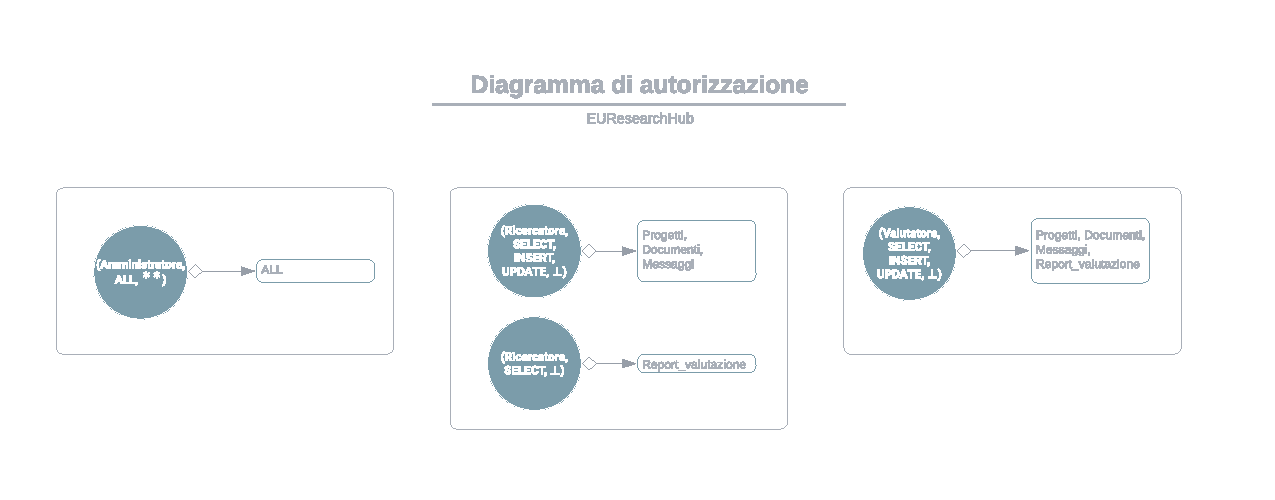
\includegraphics[scale = 0.7]{1.pdf}
\end{center}
I vantaggi di questa includono un accesso rapido al conteggio dei progetti per stato e un miglioramento delle prestazioni per le query che richiedono queste informazioni come nel caso sopra illustrato. Gli svantaggi includono un maggiore utilizzo dello spazio su disco e la necessità di aggiornare la materialized view ogni volta che i dati nella tabella \imtaInlinecode{latex}{projects} cambiano: indicamente alla fine di ogni finestra di valutazione.  Per fare fronte a questo ultimo problema abbiamo inserito un nuovo trigger \imtaInlinecode{latex}{refresh_project_status_count}, attivato solo a seguito di aggiornamento o inserimento di un nuovo status per ogni statement.  \\

\begin{minipage}{\linewidth}
\begin{imtaCode}{PostgreSQL}
CREATE FUNCTION "EUResearchHub".refresh_project_status_count()
 RETURNS trigger
 LANGUAGE plpgsql
AS $function$
BEGIN
  REFRESH MATERIALIZED VIEW projects_status_count;
  RETURN NEW;
END;
$function$

\end{imtaCode}
\end{minipage}



\end{itemize}


















.
\chapter{Implementazione back-end}
\section{Flask e SQLAlchemy}
\section{Expression Language e ORM}
\section{Sicurezza}
\subsection{Protezione da XSS}
\subsection{Protezione da SQL Injection}
\subsection{Meccanismi di sicurezza aggiuntivi}
\section{Approfondimento delle tecnologiche specifiche}
\subsection{\texttt{libreria1} }
\subsection{\texttt{libreria2} }

\chapter{Implementazione front-end}
\section{Brand identity}
\section{Demo}
\section{Approfondimento delle tecnologiche specifiche}
\subsection{\texttt{framework1} }
\subsection{\texttt{css} }
\subsection{\texttt{javascript} }

\chapter{Collaborazione e contributo individuale}
\section{Planning}
\section{Descrizione del ruolo di ciascun membro del gruppo}

In order to use this template, you simply need to have a \TeX{} distribution installed, copy this file in your working directory and add the \imtaInlinecode{latex}{\usepackage{imta_core}} command in the preamble of your top document. 
The \texttt{babel} package should be loaded first when used in combination with \texttt{imta\_core}.

If you would prefer to properly install the package once it for all instead of having multiple copies, you can do so by manually installing it. 
Since this can be a little bit tedious for a new \LaTeX{} user, we introduced a custom Python script. 
Simply run the \texttt{imta\_install.py} script and everything should be alright.
This script supports Python 2 and 3, and both Mik\TeX{} and \TeX{}Live environments. 

Note that this template is compatible with at least \TeX Live and MiK\TeX distributions, although we have noticed some issues might happen when trying to resolve dependencies with the latter. 
If so, then try to update your distribution using your Mik\TeX manager.
\footnote{See \textit{\href{https://tex.stackexchange.com/a/359851}{General Guide to Installing Packages with MikTeX Package Manager}} on \TeX Stack Exchange for more details.}


The \texttt{imta\_core} package provides a \LaTeX{} template that satisfies the IMT Atlantique corporate identity rules.
\footnote{See \textit{\href{https://intranet.imt-atlantique.fr/wp-content/uploads/2017/01/imt_atlantique_chartegraphique.pdf}{Charte Graphique}} on the IMT Atlantique's intranet for more details.} 
For slightly more advanced or specific features, you might want to refer to the \texttt{imta\_extra} package.

Since it is a package, it can be used for a variety of classes and geometry. 
It has been primarily designed to be used in \texttt{article} and \texttt{report} documents, either with \texttt{oneside}/\texttt{twoside} or \texttt{onecolumn}/\texttt{twocolumn} geometries. 
If you are not sure how to start, we invite you to have a look at the \texttt{skeleton} file provided with this template.

The \imtaInlinecode{latex}{\imtaQuestion} command outputs and formats a question counter.
It's meant to be used in reports for assignment with questions.
The counter should be reset with the \imtaInlinecode{latex}{\imtaQuestionReset}.
This couple of commands is meant to be used for sectioning when the assignment does not use a more explicit titling.


The \imtaInlinecode{bash}{imta_core} package offers a one-level-deeper section than the usual deepest \imtaInlinecode{latex}{\subsubsection}.
This provides an alternative to the usual \imtaInlinecode{latex}{\paragraph}.


The \imtaInlinecode{latex}{\chapter} command has been redefined to print the word "chapter" in front of the figure. 
This command is compatible with several languages\footnote{This functionality currently supports english, french, german, portuguese and spanish.} but requires the \texttt{babel} package to be loaded first. 
The default language is english.

This command also prints a small design on the bottom right corner of the page and updates the upper section title. 
In case the document is in \texttt{twoside} mode, it ensures the chapter page is on the right by inserting a blank page if necessary. 
In case the document is in \texttt{twocolumn} mode, it also temporarily restores a \texttt{onecolumn} geometry to print the chapter page.



The core package defines four colors, including the three colors of the IMT Atlantique, and a uniform and arbitrary gray.
These are defined as follows:

\begin{imtaCode}{latex}
\definecolor{imtaGreen}{RGB}{164, 210, 51}
\definecolor{imtaLightBlue}{RGB}{0, 184, 222}
\definecolor{imtaDarkBlue}{RGB}{12, 35, 64}
\definecolor{imtaGray}{RGB}{87, 87, 87}
\end{imtaCode}

Here are samples of these colors, with text in both black and white for previsualising the contrast.

\begin{figure}[H]
    \centering
    \resizebox{10cm}{!}{%
    \begin{tikzpicture}
        \fill[color=imtaGray] (0, 9) rectangle (6, 11);
        \fill[color=imtaGray] (7, 9) rectangle (13, 11);
        \node at (3, 10) {\LARGE \bf imtaGray};
        \node[white] at (10, 10) {\LARGE \bf imtaGray};

        \fill[color=imtaDarkBlue] (0, 6) rectangle (6, 8);
        \fill[color=imtaDarkBlue] (7, 6) rectangle (13, 8);
        \node at (3, 7) {\LARGE \bf imtaDarkBlue};
        \node[white] at (10, 7) {\LARGE \bf imtaDarkBlue};

        \fill[color=imtaLightBlue] (0, 3) rectangle (6, 5);
        \fill[color=imtaLightBlue] (7, 3) rectangle (13, 5);
        \node at (3, 4) {\LARGE \bf imtaLightBlue};
        \node[white] at (10, 4) {\LARGE \bf imtaLightBlue};

        \fill[color=imtaGreen] (0, 0) rectangle (6, 2);
        \fill[color=imtaGreen] (7, 0) rectangle (13, 2);
        \node at (3, 1) {\LARGE \bf imtaGreen};
        \node[white] at (10, 1) {\LARGE \bf imtaGreen};
    \end{tikzpicture}
    }
    \caption{Samples of the IMT Atlantique colors}
    \label{fig:imtaColors}
\end{figure}


The official IMT Atlantique styling is not really \LaTeX-ish, and takes the decision to use a sans-serif font for body text.
Therefore, the default style uses the default \LaTeX{} font settings.
However, it is possible to enable a more IMT Atlantique-compliant styling, by calling the \imtaInlinecode{latex}{\imtaSetIMTStyle} command in the preamble.

\vspace{1em}
The main aspects of the official style are:

\begin{itemize}
    \item Use of the Helvetica font for the body;
    \item Section titles in green (\imtaInlinecode{latex}{\imtaGreen}) and other heading titles in gray (\imtaInlinecode{latex}{\imtaGray});
    \item Section title in the header;
    \item Page number at the right corner of the footer.
\end{itemize}

\vspace{1em}
For comparison, the default style of the template is:

\begin{itemize}
    \item Use of the default Computer Modern font for the body;
    \item Default style for headings: all in black;
    \item Document title at the left corner and author's name at the right corner of the header;
    \item Page number at the center of the footer.
\end{itemize}


The IMT Atlantique logo can be output at the desired width with the \imtaInlinecode{latex}{\imtaLogo} command.
The latter includes an external pdf document, \imtaInlinecode{bash}{imta_logo.pdf}, that contains the official logo.
On the other hand, the \imtaInlinecode{latex}{\imtaLogoTikz} draws an approximation of the logo with the \imtaInlinecode{latex}{tikz} package.
The following is a comparison of both commands (with an added frame). Note that the current version of this template uses \imtaInlinecode{latex}{\imtaLogoTikz} for both the front and back cover.

\begin{figure}[H]
    \centering
    \fbox{\imtaLogo{5cm}}
    \fbox{\imtaLogo{5cm}}
    \caption{Comparison between \imtaInlinecode{latex}{imtaLogo} (left) and \imtaInlinecode{latex}{imtaLogo} (right)}
    \label{fig:imtaLogo}
\end{figure}


The \texttt{imtaMaketitlepage} command outputs a title page with the names of the authors, the date of writing, and the title of the document, along with the subtitle.
For this latter purpose, the \imtaInlinecode{latex}{\subtitle} command helps define a subtitle as a part of the document's metadata, and %
is used inside of the \imtaInlinecode{latex}{\imtaMaketitlepage} command.

Since the \imtaInlinecode{latex}{\author} command consists of only one field, we recommend to simply add linebreaks when declaring the authors if several people co-author a document. 
However, should you not use the IMT Atlantique style and would like to print the authors' name on one line in the default header, we introduced the \imtaInlinecode{latex}{\imtaAuthorShort} command which sets the \imtaInlinecode{latex}{\imtaTheAuthorShort} macro. 
By default, it is equal to the \imtaInlinecode{latex}{\theauthor} command, but can be redefined to be on one line only.

The version of the document can be user-specified ausing the \imtaInlinecode{latex}{\imtaVersion} command.

Moreover, you can also add one or several partner's logo on the front cover, next to the one of IMT Atlantique. 
In order to achieve this, you can simply use the \imtaInlinecode{latex}{\imtaAddPartnerLogo} command in the preamble of your document. 
The logo will be resized so that its maximum dimension is equal to the corresponding dimension of the IMT Atlantique's logo, unless instructed otherwise.



The \texttt{imtaMakeCover} command outputs a cover as the last page of the document.
This page will always be a left page in a two-side document.


\label{sec:core:quote}
In order to add beautiful quotes to your document, it is possible to use the \imtaInlinecode{latex}{\imtaQuote} environment.

\begin{imtaQuote}
Lorem ipsum dolor sit amet, consectetur adipiscing elit, sed do eiusmod tempor incididunt ut labore et dolore magna aliqua. 
Ut enim ad minim veniam, quis nostrud exercitation ullamco laboris nisi ut aliquip ex ea commodo consequat. 
Duis aute irure dolor in reprehenderit in voluptate velit esse cillum dolore eu fugiat nulla pariatur.
Excepteur sint occaecat cupidatat non proident, sunt in culpa qui officia deserunt mollit anim id est laborum.
\end{imtaQuote}



%% Dependencies
This package depends upon a number of external packages.
The use of these is explained hereafter, and the parameters each is used with are specified as well.
Furthermore, a code snippet is presented, that shows the import line and the settings of the corresponding package.


The \imtaInlinecode{latex}{geometry} package provides ways to act on the document's format.
This package defines a A4 format, with two-centimeter margins, and a top margin of an extra centimeter for the header.

\begin{imtaCode}{latex}
\RequirePackage[a4paper, margin=2cm, top=3cm]{geometry}
\end{imtaCode}


The \imtaInlinecode{latex}{graphicx} package lets input graphics and pictures into the document.

\begin{imtaCode}{latex}
\RequirePackage{graphicx}
\end{imtaCode}


The \imtaInlinecode{latex}{fontenc} package declares an encoding for the output font.
The \imtaInlinecode{bash}{imta_core} package uses a latin font whose encoding is \imtaInlinecode{latex}{T1}.

\begin{imtaCode}{latex}
\RequirePackage[T1]{fontenc}
\end{imtaCode}


The \imtaInlinecode{latex}{hyperref} package helps typeset hypertext links.
The \imtaInlinecode{latex}{hidelinks} option hides the links, but keeps them clickable.
To output a hypertext link, use the \imtaInlinecode{latex}{\hyperref} command.

\begin{imtaCode}{latex}
\RequirePackage[hidelinks]{hyperref}
\end{imtaCode}


The \imtaInlinecode{latex}{inputenc} package manages the input format.
For uniformization purpose, the \imtaInlinecode{latex}{imta} package is written for a use with Unicode.
Therefore, it is used with the \imtaInlinecode{latex}{utf8} option.

\begin{imtaCode}{latex}
\RequirePackage[utf8]{inputenc}
\end{imtaCode}


The \imtaInlinecode{latex}{fancyhdr} package is used for customizing the header and the footer.
In the default style, the body pages have the \imtaInlinecode{latex}{fancy} style, that is defined as follows:

\begin{imtaCode}{latex}
\pagestyle{fancy}
\fancyhead{}
\fancyfoot{}
\fancyhead[L]{\thetitle}
\fancyhead[R]{\imtaTheAuthorShort}
\fancyfoot[C]{\thepage}
\end{imtaCode}

A blank style, \imtaInlinecode{latex}{imtaFirstpage}, is defined to remove the header and the footer on the first page.

\begin{imtaCode}{latex}
\fancypagestyle{imtaFirstpage}{
    \fancyhf{}
    \renewcommand{\headrulewidth}{0pt}
}
\end{imtaCode}


\begin{imtaCode}{latex}
\RequirePackage{fancyhdr}
\end{imtaCode}


The \imtaInlinecode{latex}{tikz} package is used to create the decorative figures on the front cover and on the new chapter pages. 
It is also used to recreate the IMT Atlantique logo, which can be used thanks to the \imtaInlinecode{latex}{\imtaLogoTikz{<width>}} command.

\begin{imtaCode}{latex}
\RequirePackage{tikz}
\end{imtaCode}

The \imtaInlinecode{latex}{titlesec} package allows to easily redefine a section title style, using various commands such as \imtaInlinecode{latex}{\titleformat} and \imtaInlinecode{latex}{\titlespacing}.

\begin{imtaCode}{latex}
\RequirePackage{titlesec}
\end{imtaCode}


The \imtaInlinecode{latex}{titling} package creates automated front cover or title pages. 
In this package, we provide a simple wrapper with respect to the IMT Atlantique colour code and additionnal capabilities.

\begin{imtaCode}{latex}
\RequirePackage{titling}
\end{imtaCode}


The \imtaInlinecode{latex}{anyfontsize} package provides various tools to modify the formatting of sections and chapters, using the \imtaInlinecode{latex}{\chapterfont} and \imtaInlinecode{latex}{\sectionfont} commands for instance.

\begin{imtaCode}{latex}
\RequirePackage{secsty}
\end{imtaCode}



The \imtaInlinecode{latex}{enumitem} package allows to modify various properties of lists, notably its bullets. 
This was used with the \imtaInlinecode{latex}{pifont} package to produce the IMT Atlantique list rendering.

\begin{imtaCode}{latex}
\RequirePackage{enumitem}
\end{imtaCode}


Similarly to \imtaInlinecode{latex}{fontawesome}, the \imtaInlinecode{latex}{pifont} package offers multiple special characters and symbols. 
It is used along \imtaInlinecode{latex}{enumitem} to customize the lists rendering by redefining the bullets. 
It is also used to display the large quote symbols in the \imtaInlinecode{latex}{\imtaQuote} environment.

\begin{imtaCode}{latex}
    \RequirePackage{pifont}
\end{imtaCode}


The \imtaInlinecode{latex}{mdframed} package creates various frames and boxes with a lot of customization options. 
It is used for the \imtaInlinecode{latex}{imtaQuote} environment.

\begin{imtaCode}{latex}
    \RequirePackage{mdframed}
\end{imtaCode}



% List of environments
\begin{itemize}
    \item \imtaInlinecode{latex}{\imtaQuote} displays a quote in a beautiful frame as shown in section \ref{sec:core:quote}.
\end{itemize}


%% List of commands
\begin{itemize}
    \item \imtaInlinecode{latex}{\subtitle{<subtitle>}} defines a subtitle for the document, which is displayed on the front cover when using \imtaInlinecode{latex}{\imtaMaketitlepage}.
    
    \item \imtaInlinecode{latex}{\imtaSuperviser{<name>}} defines a new field for the supervisers. 
    It works in a similar fashion to the \imtaInlinecode{latex}{\author} command and is displayed on the front cover when using \imtaInlinecode{latex}{\imtaMaketitlepage}.
    
    \item \imtaInlinecode{latex}{\imtaVersion{<version>}} defines the version of the document which is displayed on the front cover.
    
    \item \imtaInlinecode{latex}{\imtaAddPartnerLogo[<options>]{<filepath>}} adds a partner's logo next to the one of IMT Atlantique on the front cover when using \imtaInlinecode{latex}{\imtaMaketitlepage}. 
    By default, its largest dimension is set to the corresponding dimension of the IMT Atlantique's logo, but it can be overrided thanks to the \imtaInlinecode{latex}{<options>} field, which is used as options for \imtaInlinecode{latex}{\includegraphics}. 
    It supports the insertion of multiple logos, adding a linebreak whenever necessary.
    
    \item \imtaInlinecode{latex}{\imtaMaketitlepage} displays the IMT Atlantique styled front cover on the current page.
    
    \item \imtaInlinecode{latex}{\imtaAuthorShort{<shortened names>}} defines shortened author names for the header in case the IMT Atlantique style is not enabled throughout the whole document.
    It works in a similar fashion to the \imtaInlinecode{latex}{\author} command.
    
    \item \imtaInlinecode{latex}{\imtaLogo{<width>}} inserts the IMT Atlantique's logo with the desired dimension by importing the \texttt{imta\_logo.pdf} document.
    
    \item \imtaInlinecode{latex}{\imtaLogoTikz{<width}} inserts the TikZ version of the IMT Atlantique's logo with the desired dimension. 
    This removes the dependency to the \texttt{imta\_logo.pdf} file.
    
    \item \imtaInlinecode{latex}{\imtaSetIMTStyle} enables the IMT Atlantique document styling throughout the whole document.
    
    \item \imtaInlinecode{latex}{\subsubsubsection{<title>}} defines another level of sectioning, which can be useful for appendices.
    
    \item \imtaInlinecode{latex}{\imtaQuestionCounter} creates a new subsection with an independant question counter (useful for a practical report).
    
    \item \imtaInlinecode{latex}{\imtaQuestionReset} resets the question counter.
    
    \item \imtaInlinecode{latex}{\imtaMakeCover} displays the IMT Atlantique styled back cover on the current page. 
    If the document is in \texttt{twoside} mode, this command will insert a blank page if necessary, to ensure the last page is on the left side.
\end{itemize}






While the \texttt{imta\_core} package provides a \LaTeX{} template that satisfies the IMT Atlantique corporate identity rules\footnote{See \textit{\href{https://intranet.imt-atlantique.fr/wp-content/uploads/2017/01/imt_atlantique_chartegraphique.pdf}{Charte Graphique}} on the IMT Atlantique's intranet for more details.} the \texttt{imta\_extra} package provides the user some slightly more advanced or specific features.

Since it is a package, it can be used for a variety of classes and geometry. It has been primarily designed to be used in \texttt{article} and \texttt{report} documents, either with \texttt{oneside}/\texttt{twoside} or \texttt{onecolumn}/\texttt{twocolumn} geometries.
If you are not sure how to start, we invite you to have a look at the \texttt{skeleton} file provided with this template.



In order to use this template, you need to have a \TeX{} distribution installed, copy this file in your working directory and add the \imtaInlinecode{latex}{\usepackage{imta_extra}} command in the preamble of your top document.

If you would prefer to properly install the package once it for all instead of having multiple copies, you can do so by manually installing it. 
Since this can be a little tedious for a recent \LaTeX{} user, we introduced a custom Python script. 
Simply run the \texttt{imta\_install.py} script and everything should be alright.
This script supports Python 2 and 3, and both Mik\TeX{} and \TeX{}Live environments. 

Since \texttt{imta\_extra} uses the \texttt{minted} package for code colouring, two extra steps are necessary to fully resolve dependencies. 
First, you need to have \texttt{Pygmentize} installed. 
If this is not the case, you can do it using Python utilitary \texttt{pip} by executing \imtaInlinecode{python}{pip install Pygments}. 
Finally, you also need to build your document with the correct options. 
If you are using pdf\LaTeX{} as your compiler, you need to add the \imtaInlinecode{latex}{--shell-escape} option.

Note that this template is compatible with at least \TeX Live and MiK\TeX distributions, although we have noticed some issues might happen when trying to resolve dependencies with the latter. If so, then try to update your distribution using your Mik\TeX manager.
\footnote{See \textit{\href{https://tex.stackexchange.com/a/359851}{General Guide to Installing Packages with MikTeX Package Manager}} on \TeX Stack Exchange for more details.}



When writing a technical report, it can be useful to write some code with syntax highlighting, which moreover matches the template colour code.
 With this idea in mind, we introduced two custom environments, based on the \imtaInlinecode{latex}{minted} package: \imtaInlinecode{latex}{\imtaCode{<language>}} and \imtaInlinecode{latex}{\imtaConsole}. 
 This means they are both \imtaInlinecode{latex}{\verbatim}-based environments (ie: the text is not interpreted by \LaTeX{} in any way).

\begin{figure}[!ht]
\begin{minipage}{.45\linewidth}
\renewcommand{\theFancyVerbLine}{\texttt{\textcolor{gray!150}{\normalsize \oldstylenums{\arabic{FancyVerbLine}}}}}%
\vspace{0.5\baselineskip}%
\begin{mdframed}[backgroundcolor=imtaCodeLinenosFrame, innerrightmargin=0pt, innertopmargin=0pt, innerbottommargin=0pt, linewidth=1pt]
\begin{mdframed}[backgroundcolor=imtaCodeBackground, skipabove=0pt, skipbelow=0pt, rightmargin=0pt, leftmargin=3ex, linewidth=0pt, innertopmargin=5pt, innerbottommargin=5pt, innerleftmargin=1ex]%
\begin{minted}[linenos, breaklines]{latex}
\begin{imtaCode}{python}
def mac(a, b, c = 0):
    # multiply-accumulate function
    return a*b + c
\end{imtaCode}
\end{minted}
\end{mdframed}
\end{mdframed}
\end{minipage}
\hfill
\begin{minipage}{.45\linewidth}
\vspace{2em}
\begin{imtaCode}{python}
def mac(a, b, c = 0):
    # multiply-accumulate function
    return a*b + c
\end{imtaCode}
\end{minipage}
\caption{Example of the \texttt{imtaCode} environment (left) and its rendering (right)\label{fig:imtaCode}}
\end{figure}


\begin{figure}[!ht]
\begin{minipage}{.45\linewidth}
\renewcommand{\theFancyVerbLine}{\texttt{\textcolor{gray!150}{\normalsize \oldstylenums{\arabic{FancyVerbLine}}}}}%
\vspace{0.5\baselineskip}%
\begin{mdframed}[backgroundcolor=imtaCodeLinenosFrame, innerrightmargin=0pt, innertopmargin=0pt, innerbottommargin=0pt, linewidth=1pt]
\begin{mdframed}[backgroundcolor=imtaCodeBackground, skipabove=0pt, skipbelow=0pt, rightmargin=0pt, leftmargin=3ex, linewidth=0pt, innertopmargin=5pt, innerbottommargin=5pt, innerleftmargin=1ex]%
\begin{minted}[linenos, breaklines]{latex}
\begin{imtaConsole}
    pwd
    grep -R "lorem" *
\end{imtaConsole}
\end{minted}
\end{mdframed}
\end{mdframed}
\end{minipage}
\hfill
\begin{minipage}{.45\linewidth}
\vspace{2em}
\begin{imtaConsole}
pwd
grep -R "lorem" *
\end{imtaConsole}
\end{minipage}
\caption{Example of the \texttt{imtaConsole} environment (left) and its rendering (right)\label{fig:imtaCode}}
\end{figure}

To further ease this process and allow the user to import code from external documents (just as figures), two commands have been introduced: \imtaInlinecode{latex}{\imtaCodeFromFile{<file>}{<language>}} and \imtaInlinecode{latex}{\imtaConsoleFromFile{<file>}}.



In long documents, in can be useful to structure the list of figures or tables by printing the highest section (chapter or section) containing the items. 
In order to achieve this, the \texttt{figure} and \texttt{table} environments have been redefined, as well as the \texttt{chapter} and \texttt{section} commands. 
The default behavior is thus to print the upper level section in the list of figures or tables. 
If you would like to disable this functionalities, you can do it by using the \texttt{nouppersectioninlof} or \texttt{nouppersectioninlot} option when loading the package. Simply type \imtaInlinecode{latex}{\usepackage[<options>]{imta_extra}} in the preamble.


In order to ease the page numbering and differentiate the preamble of your document (front cover, table of contents, list of figures, abstract, etc) from the corpus of your document, we introduced the \imtaInlinecode{latex}{\frontmatter} and \imtaInlinecode{latex}{\mainmatter}. 
They respectively set the page numbering style to roman or arabic.


%% Dependencies


The \imtaInlinecode{latex}{mdframed} package creates various frames and boxes with a lot of customization options. 
It is used for the custom code listings.

\begin{imtaCode}{latex}
    \RequirePackage{mdframed}
\end{imtaCode}


The \imtaInlinecode{latex}{minted} package provides powerful code listings tools. This package however requires the installation of the Python pakage \imtaInlinecode{text}{Pygments} as well as the compilation option \imtaInlinecode{text}{--shell-escape}. 
It is used for the custom code listings.

\begin{imtaCode}{latex}
    \RequirePackage{minted}
\end{imtaCode}



% List of environments
\begin{itemize}
    \item \imtaInlinecode{latex}{\imtaCode{<language>}} displays its content as syntax highlighted code according to the provided language and with line numbers on the side. 
    \item \imtaInlinecode{latex}{\imtaConsole} displays its content in a custom verbatim environment.
\end{itemize}


%% List of commands
\begin{itemize}
    \item \imtaInlinecode{latex}{\imtaInlinecode{<language>}{<code>}} displays its content on the current line as syntax highlighted code according to the provided language.
    \item \imtaInlinecode{latex}{\imtaCodeFromFile{<language>}{<path>}} displays the content of the given file as syntax highlighted code according to the provided language and with line numbers on the side.
    \item \imtaInlinecode{latex}{\imtaConsoleFromFile{<path>}} displays the content of a given file in a custom verbatim environment.
    \item \imtaInlinecode{latex}{\imtaFrontMatter} resets the page counter and changes its style to roman numerals.
    \item \imtaInlinecode{latex}{\imtaMainMatter} resets the page counter and changes its style to arabic numerals.
\end{itemize}


%% List of import options
\begin{itemize}
    \item \imtaInlinecode{latex}{nouppersectioninlof} disables the printing of the upper section in the list of figures
    \item \imtaInlinecode{latex}{nouppersectioninlot} disables the printing of the upper section in the list of tables
\end{itemize}


\end{document}

%%%%%%%%%% END %%%%%%%%%% 
%%%%%%%%%%%%%%%%%%%%%%%%% 
